% mainfile: ../praca_magisterska_orbifoldy.tex
%\synctex=1
\chapter{Order type and topology}\label{order structure}
%
%Order type with zanurzenie w R
%
%1537/137
%

In this chapter we will discuss that both the order type and the topology inherited from $\mathbb{R}$
of the set $\spe$ of all possible Euler orbicharacteristics 
of two-dimensional orbifolds are that of $\omega^\omega$. 
%We will call this set $\spe$.

This $\omega^\omega$ will lie in $\mathbb{R}$ in reverse order, i.e. for $x, y \in \spe$, 
such that such that $x <_{\mathbb{R}} y$, we will have $x >_{\omega^\omega} y$. 
As such, set $\spe$ will be treated as having the order type $\omega^\omega$ in the sense of 
having order type $\omega^\omega$ inherited from the reversed order in $\mathbb{R}$. 
%It will 
%be treated as such when we will be discusing order type of 
However, when referring to a particular elements of $\spe$ as "greater" or "smaller" with 
respect to each other, we will use the usual order from $\mathbb{R}$.


To determine order type and topology of $\spe$ we will first study how $\speD$ looks like. 
Then, remembering that 
$\spe = \speS \cup \speD$ and $\speS = 2\speD$ we will make an argument for $\spe$. 

%We also have shown that all possible \Eoc s are achieved without using cusps. As such, 
%we will use 
%cusps, remembering, that we can always get rid of them, if needed. So above $I_i$ and $b_j$ 
%are ranging over $\mathbb{N}_{>0}\cup \{\infty\}$, where expressions for infinity are defined as 
%a limits. The fact that it agrees with the definition of the \Eoc\ on the geometrical terms was 
%addressed in \ref{extended_Euler_orbicharacteristic}. \\
%Here is the notation that will be used: \\
%$\spe$ - spectrum of all possible \Eoc\ of two-dimentional orbifolds \\
%$\spe{M}$ - spectrum of all possible \Eoc\ of $M$ orbifolds \\

%% We would like to make some more observations concerning subsets of $\spe$. 
%% For any two-dimentional manifold $M$, observe, that:

%Now we state what we can already conclude. 


%\begin{theorem}\label{all_spectra_are_isomorphic}
%For any two two-dimentional manifolds $M$, $N$ spectras $\spe{M}$ and $\speM(N)$ have the same 
%order type and topology. 
%\end{theorem}
%\textbf{Proof} \\



\section{Order type and topology of $\speD$}


In this section we will also describe precisely where accumulation points of $\speD$ lie and of 
 which order 
(see below \ref{accumulation_points_definitions repetition} or 
\ref{accumulation_points_definitions}) they are. Analysis of locations of those 
accumulation points, as interesting as it is alone will also be necessary for providing 
our argument about order type and topology of $\speD$. 
\subsection{Definition of order of accumulation points}
\label{accumulation_points_definitions repetition} 
%\todo{zmienić to wszystko na rangę cantora bendiksona}
%We start with one technical definition of "transitive order" that will be almost what we want
%and then, there will be the the definition of "order", which is the definition that we need.
%\begin{definition}
%(Inductive). 
%%We say, that the point $a$  from the topological space $X$ is an acccumulation 
%%point of the transitive order 0, when
%We say that the point is an acccumulation point of a transitive order $0$, when it is 
%an isolated point. 
%We say that the point is an acccumulation point of a transitive order $n + 1$, when it is 
%an acccumulation point (in the usual sense) of the accumulation points of the transitive 
%order $n$. 
%\end{definition}  
%The only issue of the above definition is that the point of the transitive order $n$ 
%is also a point 
%of the transitive order $k$, for all $0< k \leq n$. We want a definition of order such that 
%for any point, there is at most one integer that is its order. So we define:
%\begin{definition}
%We say that the point is an acccumulation point of order $n$ iff it is an acccumulation point 
%of the transitive order $n$ and it is not an acccumulation point of the transitive order $n+1$. 
%If the point is an acccumulation point of the transitive order for an arbitrary large 
%$n$ we say that 
%the  point is an acccumulation point of order $\omega$.
%\end{definition}
These definitions are exactly the same as from appendix \ref{accumulation_points_definitions} and 
are repeated here only for the readers convenience.

We start with definition of being "at least of order $n$" that will be almost what we want
and then, there will be the definition of being "order", which is the definition that we need. \\
For a given set we define as follows:
\begin{definition}
(Inductive). 
%We say, that the point $a$  from the topological space $X$ is an acccumulation 
%point of the transitive order 0, when
We say that the point $x$ is an accumulation point of a set $X$ 
of order at least $0$, when it belongs to the set $X$. 
We say that the point $x$ is an accumulation point of a set 
of order at least $n + 1$, when it is 
an accumulation point (in the usual sense) of the accumulation points each of order at least 
$n$ i.e. in every neighbourhood of $x$ there is at least one accumulation point of a set $X$ 
of order at least $n$, distinct from $x$. 
\end{definition}  
%The only issue of the above definition is that the point of the transitive order $n$ 
%is also a point 
%of the transitive order $k$, for all $0< k \leq n$. We want a definition of order such that 
%for any point, there is at most one integer that is its order. So we define:
\begin{definition}
We say that the point is an accumulation point of order $n$ iff it is an accumulation point 
of order at least $n$ and it is not an accumulation point of order at least $n+1$. 
If the point is an accumulation point of order at least $n$ for an arbitrary large 
$n$ we say that 
the point is an accumulation point of order $\omega$.
\end{definition}
When we will say that a point is an accumulation point of some set without specifying an order 
then we will mean being an accumulation point in the usual sense; from the point of view 
of above definitions, that is, an accumulation point of order at least one.
%\todo{dopisać notację do punktów skupienia różnego stopnia}
%\begin{lemma}

%\end{lemma}
\subsection{Analysis of locations of accumulation points of $\speD$ with respect to their order}
%\subsubsection{Some preliminary observations}
We want to determine where exactly are accumulation points of the set $\speD$ with 
respect to their orders. 

For this we will use  
a handful of observations and lemmas. 
\begin{observation}\label{accumulation_points_are_in_the_spectrum}
Let us observe, that $\lim\limits_{n \to \infty} \Delta(^\ast n) = -\frac{1}{2}$. From that, 
we see, 
that for every point $x \in \speD$, the point $x - \frac{1}{2}$ is an accumulation point. 
Let us observe, that also, for every point $x \in \speD$, we have that $x - \frac{1}{2} 
\in \speD$, 
because $\Delta(^\ast \infty) = -\frac{1}{2}$. 
\end{observation}
%Now we will show that the order type of $\speD$ is $\omega^\omega$ and where exactly are 
%its accumulation points of which orders. For this we will use  
%a handful of lemmas. 

%\subsubsection{Finiteness lemma}
\begin{lemma}\label{finiteness_lemma}
For all $n \in \mathbb{N}_{\geq 2}$ and $x \in (-\infty, 1]$ there are only finitely 
many Euler orbicharacteristics
in the interval $[x,1] \cap \speD$ of orbifolds that have points of order equal 
at most $n$. 
\end{lemma}
\subsubsection{Proof.} 
Let $x \in (-\infty, 1]$. There can be at most $\lfloor 4(1-x) \rfloor$ orbipoints on the 
$D^2$ orbifold 
with an \Eoc\ $y \in [x,1]$ since each orbipoint decreases an \Eoc\ by at least $\frac{1}{4}$ 
and the Euler characteristic of $D^2$ is $1$. 

There are only $(n-1)^{\lfloor 4(1-x) \rfloor}$ possible sets of $\lfloor 4(1-x) \rfloor$ 
orbipoints' orders that are less or equal than $n$. Hence, there are only at most 
$(n-1)^{\lfloor 4(1-x) \rfloor}$ possible \Eoc s.


\begin{lemma}\label{first_order_lemma}
If $x$ is an accumulation point of the set $\speD$ of order $n$, then $x-\frac{1}{2}$ is a
 accumulation point of the set $\speD$ of order at least $n+1$. 
\end{lemma}
\subsubsection{Proof.}
Inductive. 

$\bullet$ $n = 0$: If $x$ is an isolated point of the set $\speD$, then $x \in \speD$. 
From that, we 
have, that points $x - \frac{k-1}{2k}$ are in $\speD$ for all $k \geq 1$, from that, that 
$x-\frac{1}{2}$ is a 
accumulation point of $\speD$. 

$\bullet$ inductive step: Let $x$ be an accumulation point of the set $\speD$ of an order 
$n > 0$. 
Let $a_k$ be a sequence of accumulation points of order $n-1$ convergent to $x$. From the 
inductive assumption, we have, that $a_k - \frac{1}{2}$ is a sequence of accumulation points 
of order at least $n$. From the basic sequence arithmetic it is convergent to $x-\frac{1}{2}$. 
From that, we have that $x-\frac{1}{2}$ is an accumulation point of the set $\speD$ of order 
at least $n+1$. $_\square$
\begin{lemma}\label{second_order_lemma}
If $x$ is an accumulation point of the set $\speD$ of order $n$, then $x+\frac{1}{2}$ is 
an accumulation point of the set $\speD$ of order at least $n-1$.  
\end{lemma}
\subsubsection{Proof.}  
Inductive 

$\bullet$ $n = 1$: We assume, that $x$ is an accumulation point of isolated points of the set 
$\speD$. 
%Let us observe
From \ref{finiteness_lemma} we know, that for all $m$ there are only finitely many 
Euler orbicharacteristics 
in the interval $[x,1]$ of orbifolds that have dihedral points of order equal at most $m$. 
%\todo{może to dać jako osobny lemat}

From that, for arbitrary small neighborhood $U \ni x$ and arbitrary large $m$ there exist 
an orbifold 
that has a dihedral point of period grater than $m$, whose Euler orbicharacteristic lies in $U$. 
Let us take a sequence of such \Eoc s $a_k$ convergent to $x$, that we can choose 
a divergent to infinity sequence of degrees of dihedral points $b_k$ of orbifolds of \Eoc s 
equal $a_k$. 
%\smalltodoII{picture} 
%\todo{Obrazek}

Let us observe, that for all $k$, the number $a_k+\frac{b_k-1}{2b_k}$ is in $\speD$. 
It is so, because $a_k$ is an \Eoc\ of an orbifold that have a dihedral point of period $b_k$, so 
identical orbifold, only without this dihedral point, has an \Eoc\ equal to $a_k + 
\frac{b_k-1}{2b_k}$. 
\begin{figure}[H]
\centering
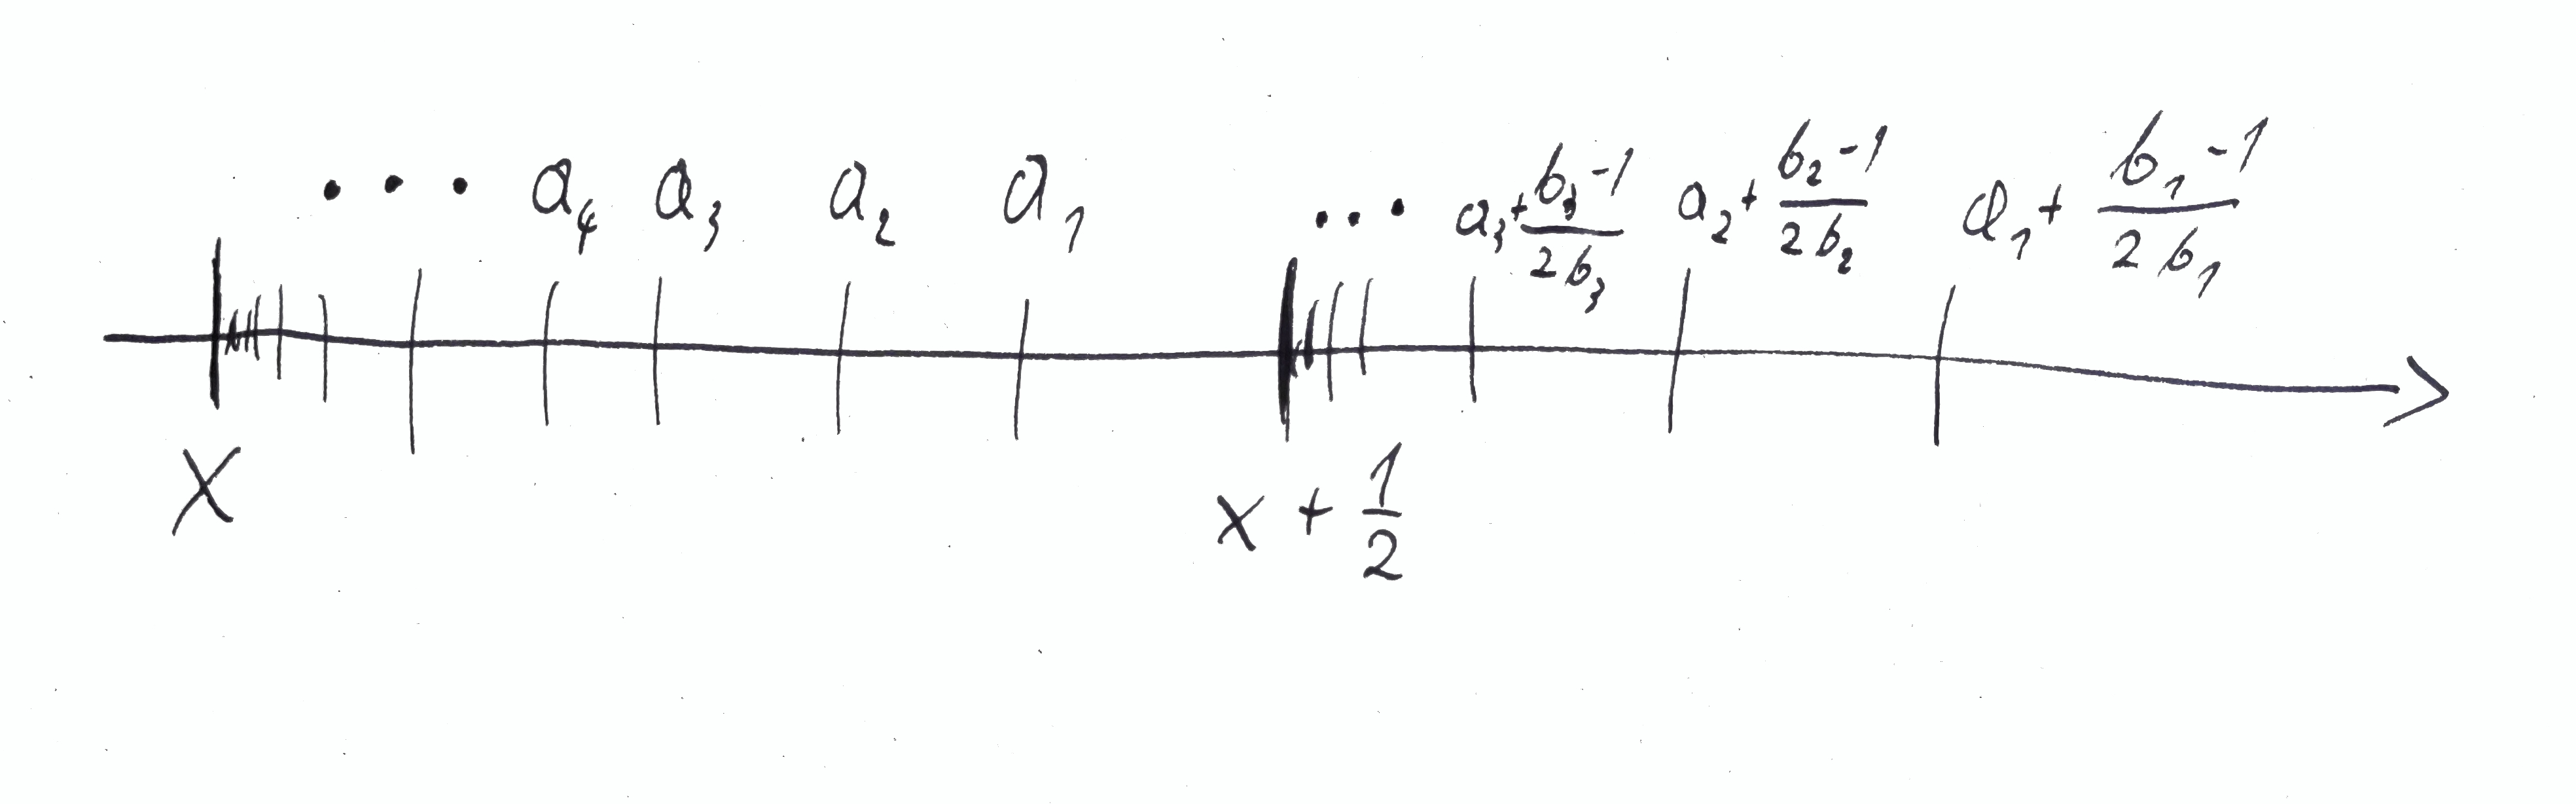
\includegraphics[width=\textwidth]{"../order_type_and_topology/x+1over2_2.jpg"}
\caption{Sequences $\{a_n\}$ and $\{a_n+\frac{b_n-1}{2b_n}\}$.}
\end{figure}
The sequence $a_k + \frac{b_k-1}{2b_k}$ converge to $x+\frac{1}{2}$. From that we have, that 
$x + \frac{1}{2}$ is an accumulation point of the set $\speD$ of order at least $0$. \\
$\bullet$ inductive step: Let $x$ be an accumulation point of the set $\speD$ of order $n > 1$. 
Let $a_k$ be a sequence of accumulation points of the set $\speD$ of order $n-1$ 
convergent to $x$. 
From the inductive assumption the sequence $a_k + \frac{1}{2}$ is a sequence of an accumulation
 points of the set $\speD$ of order $n-2$ convergent to $x + \frac{1}{2}$. From that 
 $x + \frac{1}{2}$ is an accumulation point of the set $\speD$ of order at least 
 $n-1$. $_\square$ 
\begin{lemma}\label{third_order_lemma}
If $x$ is an accumulation point of the set $\speD$ of order $n+1$, then \\
$x - \frac{1}{2}$ is an accumulation point of the set $\speD$ of order $n+2$ and \\
$x + \frac{1}{2}$ is an accumulation point of the set $\speD$ of order $n$. 
\end{lemma}
\subsubsection{Proof.} 

Let $x$ be an accumulation point of the set $\speD$ of order $n+1$. From the lemma 
 \ref{first_order_lemma} we know, that $x - \frac{1}{2}$ is an accumulation point of the set 
 $\speD$ of order at least $n+2$. Now let us assume (for a contradiction), that $x - \frac{1}{2}$ 
 is an \apots\ $\speD$ of order $k>n+2$. But then from the lemma \ref{second_order_lemma} 
 we have that $x$ is an accumulation point of the set $\speD$ of order at least $n+2$ and that 
 is a contradiction. 
 
Analogously, from the lemma \ref{second_order_lemma} we know, that $x + \frac{1}{2}$ is a 
accumulation point of the set $\speD$ of order at least $n$. Let us assume (for a contradiction), 
that $x+ \frac{1}{2}$ is an accumulation point of the set $\speD$ of order $k>n$. But then 
from the lemma \ref{first_order_lemma} we have that $x$ is an accumulation point of 
the set $\speD$ 
of order at least $n+2$ and that is a contradiction. $_\square$ 
\begin{lemma}\label{accumulation_points_of_the_set}
For all $n \in \mathbb{N}$ all accumulation points of the set $\speD$ of order $n$ are in $\speD$.
\end{lemma}
\subsubsection{Proof.}
Inductive 

$\bullet$ $n=0$: Clear, as they are isolated points of $\speD$. 

$\bullet$ inductive step: Let $x$ be a \apots\  $\speD$ of order $n>0$. From the lemma 
\ref{third_order_lemma} point $x+\frac{1}{2}$ is an accumulation point of the set $\speD$  
of order $n-1$. From the inductive assumption $x+\frac{1}{2} \in \speD$. Then, 
from \ref{accumulation_points_are_in_the_spectrum}, we have that $x \in \speD$. 
$_\square$ 

\begin{corollary}
Set $\speD$ is closed in $\mathbb{R}$.
\end{corollary}

\begin{theorem}\label{greatest \apots}
The greatest \apots\ $\speD$ of order $n$ is $1-\frac{n}{2}$.
\end{theorem}
\subsubsection{Proof.}
Inductive 

$\bullet$ $n=0$: We know, that $1\in \speD$ and $1$ is the greatest element of $\speD$. 

$\bullet$ an inductive step: From the inductive assumption we know that $1-\frac{n}{2}$ is 
the greatest \apots\ $\speD$ of order $n$. From the lemma \ref{third_order_lemma} we have then 
that $1-\frac{n+1}{2}$ is a \apots\ $\speD$ of order $n+1$. Let us assume (for a contradiction), 
that there exist a bigger accumulation point of order $n+1$ equal to $y > 1-\frac{n+1}{2}$. 
But then, from lemma \ref{third_order_lemma}, point $y+\frac{1}{2}$ would be an accumulation 
point 
of order $n$, what gives a contradiction, because $y+\frac{1}{2}>1-\frac{n}{2}$. $_\square$ 
\\[8pt]
From the above discussion we can also formulate following corollary that will be useful later: 
% corollary (stated in for deifferent ways 
%as one are sometimes more useful that another): 
%\begin{corollary}\label{predescors}
%Let $x \in \spe$. Then there exists $n \in \mathbb{N}$ such that $x + \frac{n}{2} \in \spe$ 
%but $x+\frac{n+1}{2} \not\in \spe$. For such $n$ we have that $x$ is an \apots\ $\spe$ of 
%order $n$.  
%\end{corollary}
%\begin{corollary}
%\end{corollary}
%%Above corollary can be refolmulated in a way that sometimes is more useful:
%\begin{corollary}\label{predescors_variant_II}
%Let $x \in \spe$ be an \apots\ $\spe$ of order $n$. Then there is $y \in \spe$ that is 
%an isolated point of $\spe$ such that $x = y - \frac{n}{2}$.   
%\end{corollary}
\begin{corollary}\label{predescors}
Let $x \in \speD$. Then:
\begin{itemize}
\item there exists $n_1 \in \mathbb{N}$ such that $x + \frac{n_1}{2} \in \speD$ 
but $x+\frac{n_1+1}{2} \not\in \speD$. 

In other words, there exist $y \in \speD$ and 
$n_1 \in \mathbb{N}$ such that 
$y + \frac{1}{2} \not\in \speD$ and such that $x = y - \frac{n_1}{2}$;
\item there exists $n_2 \in \mathbb{N}$ such that $x$ is an \apots\ $\speD$ of 
order $n_2$
%\item $x$ is an \apots\ $\speD$ of order $n_2$, for some $n_2 \in \mathbb{N}$;  
\end{itemize}
and $n_1 = n_2$.
\end{corollary}

\subsection{Proof that $\speD$ is well ordered}

\begin{definition} 
Let $B_0 = \{1\}$.
For an $n \in \mathbb{N}_{>0}$, let $B_n$ be the set of all possible \Eoc\ realised 
by orbifolds of type 
$*^*b_1, \cdots, ^*b_n$. For a given $n$ these are 
$D^2$ orbifolds with precisely $n$ non trivial orbipoints on their boundary.
\end{definition}


\begin{observation}\label{recursive_relation}
There is a recursive relation, that $B_{n+1}=B_n+\{-\frac{n-1}{2n}\ |\ n\geq 2\}$
\end{observation}
\subsubsection{Proof.}
It is so, because every orbifold with $n+1$ orbipoints can be obtained by adding one point 
to an orbifold with $n$ orbipoints and the set 
$\{-\frac{n-1}{2n}\ |\ n\geq 2\} = \{\Delta(^\ast b)\ |\ b \geq 2\}$. $_\square$
%Let take $x \in B_{n+1}$. Then there exist some orbifold $O_1$ with an \Eoc\ equal to $x$ with 
%signature $\ast b_1, \cdots, b_{n+1}$. 
%Taking an orbifold $O_2$ with signature $\ast b_1, \cdots, b_n$, its \Eoc\ $\cho{O_2}$ 
%is in $B_n$ as $O_2$ has $n$ orbipoints. The difference between $\cho{O_1}$ and $\cho{O_2}$ 
%is $-\frac{b_{n+1} - 1}{2b_{n+1}} \in \{-\frac{n-1}{2n}\ |\ n\geq 2\}$. \\
%Let take $x \in B_n+\{-\frac{n-1}{2n}\ |\ n\geq 2\}$. Then $ x = x_n + x'$ for some 
%$x_n \in B_n$ and $x' \in \{-\frac{n-1}{2n}\ |\ n\geq 2\}$. Let 


\begin{observation}\label{form_of_a_spectrum}
Observe that, as any orbifold has only finitely many orbipoints, we have that $\speD \subseteq 
\bigcup\limits^\infty_{n=0}B_n $. We defined $\speD$ as a set of all possible \Eoc\ of disk 
orbifolds, so $\speD \supseteq 
\bigcup\limits^\infty_{n=0}B_n $. From this we have that $\speD = \bigcup\limits^\infty_{n=0}B_n$.
\end{observation}

\begin{lemma}\label{fixed_number_of_orbipoints}
For any given $n \in \mathbb{N}$ the set $B_n$ is a subset of the interval 
$[1-\frac{n}{2}, 1-\frac{n}{4}]$.
\end{lemma}
\subsubsection{Proof.}
Take $x \in B_n$. There exists an orbifold $O$ with signature $\ast b_1, \cdots, b_n$, 
such that $\cho{O} = x$. We have that $\forall_i -\frac{1}{2} \leq \Delta(^*b_i) \leq 
-\frac{1}{4}$. From this $-\frac{n}{2} \leq \Delta(^*b_1, \cdots, ^*b_n) \leq -\frac{n}{4}$, 
so $\cho{O} \in [1-\frac{n}{2}, 1-\frac{n}{4}]$. $_\square$

\begin{observation}\label{ascending_in_B_n}
From \ref{recursive_relation} and \ref{two_sets_lemma}, we have that $B_n$ do not have 
infinite ascending sequence for all $n$. 

Further, from \ref{sum_lemma} we conclude, 
that $\bigcup\limits_{n=0}^N B_n$ do not have infinite ascending sequence for all $N$.
\end{observation}

\begin{theorem}\label{well_order}
In $\speD$ there are no infinite strictly ascending sequences, hence, it is well ordered.
\end{theorem}
\subsubsection{Proof.}
%Being well ordered is a consequence of not having infinite strictly ascending sequences. 
For the sake of contradiction lets assume that $c_n$ is an infinite strictly ascending sequence in 
$\speD$. As $c_n$ is bounded from below by $c_0$ and whole $\speD$ is bounded from above 
by $1$, all elements of $c_n$ are in the interval $[c_0, 1]$. 
From \ref{form_of_a_spectrum} we have, that $\speD = \bigcup\limits^\infty_{n=0}B_n$. 

Lemma 
\ref{fixed_number_of_orbipoints} says that for all $n$ we
have $B_n \subset [1-\frac{n}{2}, 1 - \frac{n}{4}]$. From this, we know, that for any 
$n$ such that $1 - \frac{n}{4} < c_0$ 
we have, that $B_n \cap [c_0,1] = \varnothing $. Let $n_0$ be the smallest such that 
$1 - \frac{n_0}{4} < c_0$ (so $n_0 > 4(1-c_0)$). 
Then for all $n > n_0$ we have $1 - \frac{n}{4} < c_0$, meaning, that 
for all $n > n_0$ we have
$B_n \cap [c_0,1] = \varnothing $, so all elements of $c_n$ are in 
$\bigcup\limits_{n=0}^{n_0} B_n$.
But this contradicts \ref{ascending_in_B_n}.  $_\square$
%\todo{rozwinąć ostatni argument}









\subsection{Proof that order structure and topology of $\speD$ are those of $\omega^\omega$}
%\smalltodoII{rozbić to na dwa?} 
\begin{theorem}\label{speD_order_type}
Order type and topology inherited from $\mathbb{R}$ of $\speD$ are $\omega^\omega$. 
\end{theorem}
\subsubsection{Proof.} 
%that order type of $\speD$ is $\omega^\omega$: \\
%- proof that it is at least $\omega^\omega$ \\

We will first prove, that the order type of $\speD$ is $\omega^\omega$.

$\bullet$ Order type of $\speD$ is at least $\omega^\omega$.

%For the sake of contradiction, let us suppouse that the order type $\eta$ of $\speD$ 
%is less than $\omega^\omega$. Then $\eta$ is smaller than $\omega^n$ for some $n$. 
%However, 
From \ref{greatest \apots} we know, that for every $n\in \mathbb{N}$, in $\speD$ there are 
accumulation points of order $n$. From this, and from \ref{accumulation_points_and_order} 
we know that $\speD$ has an order type at least $\omega^n$, for all $n\in \mathbb{N}$. 
The smallest ordinal number equal at least $\omega^n$, for all $n \in \mathbb{N}$ is 
$\omega^\omega$. Thus, the order type of $\speD$ is at least $\omega^\omega$.\\
% but for sufficiently distant have accumulation point. \\
%done \\

$\bullet$ Order type of $\speD$ is at most $\omega^\omega$.

%- proof that it is at most $\omega^\omega$\\
For the sake of contradiction, let us suppose, that the order type $\eta$ of $\speD$ is 
strictly greater than $\omega^\omega$. Then, $\speD$ has a set $A$ of an order type 
$\omega^\omega$ as it's prefix. The set $A$ is bounded, as the $\omega^\omega+1$st element of 
$\speD$ is greater than any element of $A$. 
Let $n$, be such that $1-\frac{n}{2}$ is smaller than any element of $A$. 
As $A$ is of order type $\omega^\omega$ it has a prefix $B$ of order type $\omega^n$.
From \ref{accumulation_points_and_order} we know, that $B$ has an accumulation point $b$ 
of order $n$. This gives us a contradiction, as $b > 1-\frac{n}{2}$, and from \ref{greatest \apots} 
we know, that $1-\frac{n}{2}$ is the greatest accumulation point of order $n$ in $\speD$. \\

%suppouse it is bigger \\
%then there is a point before which there is omega omega order \\
%wooo, but it cant be since first with accumulation is at something spmething \\
%done \\
%ok, so how to give convincing correspondence between accumulation points and $\omega^n$??
%Lemma \\
%there cant be order of type \\
%i wish I can cite this from somewhere \\ 
%
%\newpage
%

Now, we will prove, that the topology inherited from $\mathbb{R}$ 
on $\speD$ is that of $\omega^\omega$.

From \ref{accumulation_points_of_the_set} we know that every accumulation point 
of $\speD$ is in $\speD$. 
%We just showed, that the order type of $\speD$ is $\omega^\omega$.
Thus, $\speD$ satisfies the assumptions of the lemma \ref{order_preserving_homeomorphism_theorem} 
and 
%\ref{accumulation_points_of_the_set} and the first part of the proof, that just showed, 
%that the order type 
we have that 
the topology of $\speD$ inherited from $\mathbb{R}$ is $\omega^\omega$. 






%\section{Order type and topology of $\spebr{M}$}\label{all_spectra_are_isomorphic}\label{spe_M}






%In short, for every manifold it either have 

\section{Order type and topology of $\spe$}
\begin{theorem}
The order type of the set and topology inherited from $\mathbb{R}$ 
of the set of possible Euler orbicharacteristics of two-dimensional orbifolds  
$\spe$ is $\omega^\omega$. 
\end{theorem}
\subsubsection{Proof.}
From \ref{sufficiency of D2 and S2}
%\ref{sum of spectras} 
we know, that $\spe = \speD \cup \speS$.

From \ref{speD_order_type} and \ref{2times homeomorphism}, we have that order types and 
topologies of $\speD$ and $\speS$ both are $\omega^\omega$ and that $\speS = 2\speD$.  

We will now prove that the order type of $\spe$ is $\omega^\omega$.

From \ref{greatest \apots} we know, that the largest \apots\ $\speD$\ of order $n$ is 
$1-\frac{n}{2}$. From, this and from the fact that $\speS = 2\speD$ we know that 
that the largest \apots\ $\speS$\ of order $n$ is 
$2-n$. 

From this, we have, that for every $m \in \mathbb{N}_{>0}$, order type of 
$(-m, \infty) \cap \speD$ is $\omega^{2m+2}$ and that order type 
of $(-m, \infty) \cap \speS$ is $\omega^{m+2}$ (if $-m = 1-\frac{n}{2}$, then 
$n = 2m + 2$ and 
%simmilarly 
if $-m = 2 - n$, then $n = m + 2$). 
%So, for every $m \in \mathbb{N}_{>0}$, the order type of $\speD$ is strictly greater than 
%th

Thus, for every $m \in \mathbb{N}_{>0}$, we have that $(-m, \infty) \cap \speD$ and 
$(-m, \infty) \cap \speS$ satisfies assumptions of \ref{key_lemma}, thus, we have that 
$(-m, \infty) \cap (\speD\cup\speS)$ have an order type $\omega^{2m+2}$. 

From this we have that 
\begin{equation}
\spe = \speD \cup \speS = 
\bigcup\limits_{m=1}^\infty \left( (-m, \infty) \cap (\speD\cup\speS) \right)
\end{equation} 
have an order type $\omega^\omega$.

Now we will prove, that the topology inherited from $\mathbb{R}$ on $\spe$ 
is that of $\omega^\omega$.

We have that for $\speD$ \rba{$\speS$} every accumulation point of 
$\speD$ \rba{$\speS$} is in $\speD$ \rba{$\speS$}. From this and from 
\ref{derivative and sum is commutative} we have, that all accumulations points of $\spe$ 
are in $\spe$. From this, from lemma \ref{order_preserving_homeomorphism_theorem} we have 
that the topology of $\spe$ is $\omega^\omega$. $_\square$ 

%powiedziec, że wtedy zletmatu suma będzie też taka

%powiedzieć że w takim razie calosć będzie taka

%there are no new accumulation points -- all accumulations points are in sigma -- topology is ok

%and 
%dopisać w apendiksie, że jak wysumuję dwa o różnym typie porządkowym, to wychodzi większy równy
%Provide some argument about being homeomorphic 
%\subsubsection{Proof.}
%From \ref{speD_theorem} we know, that $\speD$ is homeomorphic with $\omega^\omega$. From 
%\ref{all_spectra_are_isomorphic}, we know, that $\speS$ is homeomorphic 
%with $\omega^\omega$. \\
%$\speS = 2\speD$, so for all $n\in \mathbb{N}$ set $\speS \cap [2,-n)$ has a lower order type then 
%$\speD\cap [2,-n)$. From this and from \ref{sum_lemma}, we have that $\speS \cup \speD$ 
%has an order type of $\omega^\omega$. \\
%For homeomorphicity, the proof of theorem \ref{speD_theorem} works as well in this case.
%$_\square$ \\[4pt]

%\section{Order type and topology of n-th cantor bendixon derivative of $\spe$ and $\spebr{M}$} 
%$\spe^{(n)}$ \\
%taking limit points is the order type of $\omega^\omega$ but not homeomorphic anymore. 
%\todo{lemat o braku nowych punktów}



%\section{Which points are in the $\spe$?}

%Here we will try to understand better the conditions that let us determine wether the point 
%lie in $\spe$ or not.
% We will also state some observations about reasoning which points 
%belong to $\spe$ based on the knowlegde of other points belonging there. \\


\section{More about how this $\spe$, $\speS$ and $\speD$ lie in $\mathbb{R}$}
This section consists of rather loose assembly of remarks and observations about some 
relations between $\spe$, $\speS$, $\speD$ and how they all lie in $\mathbb{R}$.
%\todo{movve to some other section maybe}

\begin{observation}
The first (greatest) negative \apots\ of $\spe$ is 
$-\frac{1}{12}$. It is the accumulation point of order $1$. 
\end{observation}
\subsubsection{Proof.} 

We will show, that $-\frac{1}{12}$ is the greatest negative accumulation point of the set $\speD$. 
From this we will obtain the thesis, as the set of all possible Euler orbicharacteristics 
of two-dimensional orbifolds is equal to $\speS \cup \speD$ and $\speS = 2\speD$, so 
the greatest negative point of the set $\speS$ is smaller than the greatest negative accumulation 
point of the set $\speD$. 

$\bullet$ $-\frac{1}{12}=\chi^{orb}((2,3))-\frac{1}{2}$, from this, from 
\ref{third_order_lemma}, we have that $-\frac{1}{12}$ 
an accumulation point of the set $\speD$ of order at least $1$. 

$\bullet$ Let us assume for a contradiction, that there exist bigger, negative 
accumulation point of the set $\speD$ of order at least $1$. Let us denote it by $x$. 

However, then, from the lemma \ref{third_order_lemma} point $x+\frac{1}{2}$ is 
the accumulation 
point of 
%in
the set $\speD$. What is more, since $x\in (0, -\frac{1}{12})$, then $x+\frac{1}{2} 
\in (\frac{1}{2}, \frac{5}{12})$. From the lemma \ref{accumulation_points_of_the_set} we 
have that $x$ is in $\speD$. But orbifolds of the type $\ast d_1$ can have \Eoc\ only greater or 
equal $\frac{1}{2}$. Orbifolds of the type $\ast d_1d_2$ can only have \Eoc\ $\frac{1}{2}$, 
$\frac{5}{12}$ and some smaller. Orbifolds of the type $\ast d_1d_2d_3\cdots$ can have \Eoc\ only 
lower than $\frac{1}{4}$. This analysis of the cases leads us to the conclusion, that 
$(\frac{1}{2},\frac{5}{12})\cap \speD=\emptyset$ and to the contradiction. 

$\bullet$ Above analysis of the cases leads us also to the conclusion, that $\frac{5}{12}$ 
is 
an isolated point of the set $\speD$, from this $-\frac{1}{12}$ is an accumulation point 
of order $1$ of the set $\speD$. $_\square$ 

%Let us observe, that this is a variant of Hurwitz theorem for non-compact manifolds. 
%This can be formulated as following corollary:
%\begin{corollary}

%\end{corollary}
%\subsubsection{Proof.}
\subsection{Saturation theorem}
\begin{theorem}\label{saturation theorem}
For any rational number $\frac{p}{q}$, for any two dimensional manifold $M$
there exists $N\in\mathbb{Z}$ such that 
for all $n \geq N$, we have that $\frac{p}{q} - n \in \spebr{M}$.
\end{theorem}
\subsubsection{Proof.}
Let us take $\frac{p}{q} \in \mathbb{Q}$. 
From \ref{Egyptian_fractions}, 
%after \cite{every number is expressible 
%as an egyptian fraction} 
we know that every rational number is expressible as an Egyptian 
fraction. 
%(it is true for usual definition and for our less strict definition, we can always have 
%$\frac{m}{n} = \underbrace{\frac{1}{n}+\cdots+\frac{1}{n}}_{m\ \mathrm{times}}$). 
Let us name the number of summands in some Egyptian fraction of $\frac{p}{q}$ 
as $k$. From \ref{from Egyptian fractions} we know that then 
$\chi(M) - k + \frac{p}{q} \in \spebr{M}$. From \ref{accumulation_points_are_in_the_spectrum} 
and \ref{all_spectra_are_isomorphic} we also know, 
that if $x \in \spebr{M}$, then $x - l\in\spebr{M}$, for any $l \in \mathbb{N}_0$. 
From this, we have, that 
%if $\chi(M)-k \leq 0$, then 
$k-\chi(M)$ is our $N$. 
%from the theorem and 
%the proof is finished. If $\chi(M)-k > 0$, we can take as $N$ 
$_\square$
%\todo{dokończyć}
%\begin{corolarry}
%The following theorem tells us that for any denumerator, from a sufficiently distant 
%point all rational number with this denumerator are in $\speS$.
%\begin{corollary}
%For any $d \in \mathbb{N}_{>0}$, there exists an $a_d \in \mathbb{R}$, such that for 
%any $\frac{w}{d} < a_d$, where $w \in \mathbb{Z}$, we have that $\frac{w}{d} \in \speS$.
%\end{corollary}
%\subsubsection{Proof.}
%$_\square$
%The following theorem tells us, that modulo $1$, every rational number is in $\speS$.
%\begin{theorem}
%For any rational number $\frac{p}{q}$, there exist $w \in \mathbb{Z}$ such that 
%$\frac{p}{q} + w \in \speS$.
%\end{theorem}
%\subsubsection{Proof.}
%From \ref{Egyptian_fractions}, we know that \cite{every number is expressible 
%as an egyptian fraction}
%$_\square$

\begin{corollary}\label{Saturation theorem corollary}
For any finite set of rational numbers $\{(\frac{p}{q})_i\}_{i=1}^k$, for any 
finite set of two dimensional manifolds $\{M_j\}_{j=0}^l$, there exists 
a $N\in\mathbb{N}_0$ such that 
for all $n \geq N$, for all $i\in \{1 \dots k\}$, 
for all $j\in\{1\dots l\}$ we have that  $(\frac{p}{q})_i - n \in \spebr{M_j}$.
\end{corollary}
\subsubsection{Proof.}
For each pair of $(\frac{p}{q})_i$ and $M_j$ we apply \ref{saturation theorem}, 
obtaining $N_{i,j}$. 
we take $N$ as a minimal from $\{N_{i,j}\}_{i\in\{1\dots k\}, j\in \{1\dots l\}}$. $_\square$ 

\subsection{Connections between $\speS$ and $\speD$}\label{D_and_S}
In this section we would like to 
%develop the tools and 
answer some questions about 
%interrelationships
relations between $\speS$ and $\speD$. 

%The first, stated in \ref{} is that $2\speD=\speS$. 
%This tells us all about simmilarities of their topological structures -- namely, 
%they are the same, 
%but it does not directly answers questions about how they lie in $\mathbb{R}$, relative 
%to each other.
%\subsubsection{Some preliminary observations}
%\todo{dopisać trochę inną motywację}
%\\[16pt]
From \ref{neccessity of d2 and s2} we know that both $\speS$ and $\speD$ are necessarily 
in expressing $\spe = \speS \cup \speD$. It is shown by giving examples of two points 
one from $\speS \setminus \speD \ni 2$ and one from $\speD \setminus \speS \ni -\frac{1}{84}$.
We found it interesting to ask further questions about the sets  
$\speS \setminus \speD$ and $\speD \setminus \speS$ such as what points 
exactly lie in one of $\speS$ and $\speD$ and not in the other, does it have 
any connection to the previously described order and topological structure 
or if the $\speS$ and $\speD$ 
overlap from some sufficiently distant point. This subsection is a meager attempt to 
answer some of these questions.
%\begin{corollary}
%From \ref{Saturation theorem corollary} it follows that $\speS$ and $\speD$ coincide 
%from a sufficiently distant point on any set of the form $A-n$, where $A$ is a 
%finite set of rational numbers, and $n\in\mathbb{N}$. 
%\end{corollary}
%\subsubsection{Importance of $-\frac{1}{84}$ and $-\frac{1}{42}$}
%%//Why it is how it is//
%As described in \ref{największy orbifold} we know that $-\frac{1}{84}$ is 
%the greatest possible negative \Eoc for an two dimensional orbifolds. 
%As described in \ref{największy orbifold} 
%we know that because of that $-\frac{1}{84}$ can't be in $\speS$. 
%This provides us an example of a point that is in $\speD$ but not in $\speS$, showing that 
%including $\speD$ in the statement $\spe = \speS \cup \speD$ is neccessery.

%We can ask further questions 
%\subsection{All the accumulation points of the $\speS$ are in $\speD$}

%\begin{observation}

%\end{observation}
\subsubsection{Accumulation points of the $\speS$}
We will first state some observations that will be useful in this subsubsection.
\begin{observation}
If an \Eoc\ $x$ is an accumulation point of order $n$ in $\speD$ \rba{respectively $\speS$}, 
then there exist an $D^2$ \rba{resp. $S^2$} 
orbifold with $n$ dihedral \rba{resp. rotational} points with that \Eoc. 
\end{observation}
%prrof. from chapter 3. (todo: dopisać)
\subsubsection{Proof.}
From \ref{predescors}, we know, that then $x + \frac{n}{2} \in \speD$ 
\rba{resp. $x + n \in \speS$}. 
Let $O$, be an orbifold with \Eoc\ equal to $x+\frac{n}{2}$ \rba{resp. $x+n$}. 
Then $O$ with $n$ dihedral \rba{resp. rotational} orbipoints of degree $\infty$ 
added is the orbifold we are looking for.  
\begin{observation}\label{adding_multiplied_differences}
If $x \in \speD$ \rba{respectively $\speS$}, then $1-x$ \rba{resp. $2-x$} is 
a difference in 
\Eoc\ resulting 
from some set of dihedral \rba{resp. rotational} points. From that $1-n(1-x) \in \speD$ \rba{resp. 
$2-n(2-x)\in \speS$}
for all $n \in \mathbb{N}$. 
\end{observation}
\begin{theorem}\label{all acc S in D}
All accumulation points of the $\speS$ are in $\speD$.
\end{theorem}
There are two proofs of this theorem showing nice correspondence -- one arithmetical and 
one geometrical. 
%\\
%\textbf{Proof I.}
%%\subsubsection{Arithmetical reason}
%\textbf{Arithmetical reason} \\
\subsubsection{Proof I. Arithmetical reason}
We assume that $x \in \speS$ is an \apots\ $\speS$.

%If $x \in \speS$, then $\frac{x}{2} \in \speD$. Then $1 - \frac{x}{2}$ 
%is a difference in \Eoc\ resulting from some set of cone points. We can add to the disc twice as 
%many cone points and resulting orbifold $\mathcal{O}$ will have an \Eoc\ equal to 
%$1 - 2(1-\frac{x}{2}) = x - 1$. From \ref{third_order_lemma} for the thesis it is sufficient 
%to $x - 1$ to be an \apots\ $\speD$ of order at least two. \\
%%$2-x$ is a difference in \Eoc\ resulting from some set of gyration points. We can 
%We asumed that $x \in \speS$ is an \apots\ $\speS$, so, 
By \ref{2times homeomorphism} we have, that 
$\frac{x}{2} \in \speD$ is an \apots\ $\speD$. From \ref{third_order_lemma} we have that 
$\frac{x}{2} + \frac{1}{2} \in \speD$. From that, from \ref{adding_multiplied_differences} 
we have, 
that \begin{equation}
1-\overbrace{2}^{\substack{"n"\rm\ from\ \\ 
\rm \ref{adding_multiplied_differences}}} 
(\ \overbrace{1-(\frac{x}{2}+\frac{1}{2})}^{\substack{"1-x"\rm\ 
from\ \\ \rm \ref{adding_multiplied_differences}}}\ ) \in \speD.
\end{equation} 
But $1 - 2(1-(\frac{x}{2}+
\frac{1}{2})) = x$, so $x \in \speD$. $_\square$
% for some $y \in \speD$, so $\speD$.
%\\[2pt]
%\textbf{Proof II.}
%\subsubsection{Geometrical reason}
%\textbf{Geometrical reason} \\
\subsubsection{Proof II. Geometrical reason}
We assume that $x \in \speS$ is an \apots\ $\speS$.

%If $x \in \speS$
From \ref{predescors} and \ref{2times homeomorphism} 
we know, that $x$ can be expressed as $y - 1$ for some $y \in \speS$.
Let $\mathcal{O}$ be an orbifold with the base manifold $S^2$, such that $\cho{\mathcal{O}} 
= y$. 
Let $\mathcal{O}_c$ be the orbifold created from $\mathcal{O}$ by adding one cusp. 
Then $\cho{\mathcal{O}_c} = y - 1 = x$. Topologically $\mathcal{O}_c$ with the cusp point 
removed 
%(which do not change an orbicharacteristic) 
is $\mathbb{R}^2$. 
We can compactify it with $S^1$. This operation of removing cusp point and replacing it by $S^1$ 
will not change an \Eoc\ since $\cho{S^1} = 0$, 
\Eoc\ is additive and $\Delta(\infty) = \Delta(\ast) = 1$.

What we get is an orbifold $\mathcal{O}_D$ with the base 
manifold $D^2$ and the same 
orbipoints as $\mathcal{O}$. Since orbipoints of $\mathcal{O}$ create a difference 
in \Eoc\ equal to $2-y$, we have that $\cho{\mathcal{O}_D} = 1 - (2-y) = y - 1 = x$. 
We can then replace all orbipoints from the interior of $\mathcal{O}_D$ by twice as many 
of the same degrees on its boundary \ref{moving from interior to boundary}, 
so $x \in \speD$. $_\square$\\




%The first equstion we can tackle is steaming from the chapter \ref{order structure} 
%and it is -- 
%Do $\speD$ and $\speS$ coincide? It is easy to answer that $\speD \neq \speS$ 
%(and we will do that along some harder questions in the moment), but do they coincide 
%starting from a sufficiently distant point? Or maybe, for every denominator, do they coincide 
%from a sufficiently distatn point? (Yes.) \\





